%%%%%%%%%%%%%%%%%%%%%%%%%%%%%%%%%%%%%%%%%%%%%%%%%%%%%%%%%%%%%%%%%%%%%%%%
%                                                                      %
% LaTeX, FIIW thesis template: The IB3/EE3 version                     %
%                                                                      %
%%%%%%%%%%%%%%%%%%%%%%%%%%%%%%%%%%%%%%%%%%%%%%%%%%%%%%%%%%%%%%%%%%%%%%%%
% The document format below can be used for a distributable PDF or when you print single sided
%\documentclass[11pt,a4paper,oneside]{book}
% If you want to print your thesis double-sided on paper, you can use the settings below
%\documentclass[11pt,a4paper]{book}

% For Campus GroepT use the two-column paper layout
\documentclass[11pt,a4paper,twocolumn]{report}

%%% Load the FIIW template
%%% You should specify your campus : groept, denayer, gent, geel and brugge are implemented
%%% You can hide parts of the preface by specifying some option:
%%% e.g. : noacknowledgements, noabstract, nosamenvatting, nolistoffigures, nolistoftables, nolistofsymbols
\usepackage[groept]{fiiw}


%%% Load some other basic packages
\usepackage[dutch,english]{babel}
\usepackage[latin1]{inputenc}           % needed if you have special characters in your text
%\usepackage[utf8]{inputenc}            % if your text is encoded in utf8 (and not latin1) use this package

\usepackage{natbib}						% used for cites from the bib file in your text
\usepackage{listings}             		% used for displaying source code (java, c, matlab,...)
\usepackage{verbatim}					% used for inline formatting of source code, terminal commands, ...
\usepackage{hyperref}					% include hyperlinks in the resulting PDF
\usepackage{url}						% add url's with \url{http://}
\usepackage{amsmath}					% extend math features
\usepackage[final]{pdfpages}            % include pdf's e.g.: a paper or a poster
\usepackage{float}                      % adds [H] to figure env. Puts a figure where you want it e.g. \begin{figure}[H]
\usepackage{longtable}					% used for tables that strech over muliple pages
\usepackage[toc, acronyms]{glossaries}	% used by the list of symbols

% generate lorum ipsim text in template
\usepackage{lipsum}

%%% configure layout for source code listings
%\definecolor{keyword}{rgb}{0.3,0.3,0.3}
%\definecolor{string}{rgb}{0.7,0.7,0.7}
\lstset{
	language = Java,
	basicstyle=\scriptsize\ttfamily,
	numbers=left,
	numberstyle=\tiny,
	tabsize=2,
	showspaces=false,
	frame=single,
	breaklines=true,
%	keywordstyle=\bfseries\color{keyword},
%	stringstyle=\color{string},
	extendedchars=true,
	xleftmargin=0.3\linewidth,
	xrightmargin=0.1\linewidth
}

%%% abstract, acknowledgements and list of symbols are located in another file
%%% list the filenames where you created them. If you omit one of these the page
%%% is not displayed
\acknowledgementsfile{chapters/acknowledgements}	% .tex file with acknowledgements
\abstractENfile{chapters/abstract}					% .tex file with EN abstract (in English)
%\abstractNLfile{chapters/samenvatting}				% .tex file with NL abstract (in Dutch, for Dutch students only)
\listofsymbolsfile{chapters/symbols}				% .tex file with list of symbols

%%% select the main language of your document (default = dutch)
%%% (you can select a different language for the cover page below)
%\documentlanguage{dutch}
\documentlanguage{english}

%%% if the cover page needs to be a different language as the main document, this can be set
%%% if you do not specify a coverlanguage, the cover will have the same langugage as the document
%\coverlanguage{dutch}

%%% information about you, your thesis, supervisor, ...
\program{Engineering Technology: Electronics and ICT Engineering}
\title{Project Sunflower}
\subtitle{Energy 2}
\firstnameA{Yaoqing}
\lastnameA{Tuu}
\firstnameB{Hugo}
\lastnameB{Alonso}
% BEGIN EE3 more names in a team
\firstnameC{Xin}
\lastnameC{Huang}
\firstnameD{Davit}
\lastnameD{Domuzashvili}
\firstnameE{Arthur}
\lastnameE{Dubois}
% END EE3 more names in a team
\academicyear{2024-2025}
% Supervisor is your EE3 coach
\supervisor{Gil Vranken}
\supervisorEmail{gil.vrankenh@kuleuven.be}


\begin{document}

	\preface
	\chapter{Introduction}
The advent of the 21st century has been characterized by an urgent global need to reduce dependency on fossil fuels, both to combat climate change and to build a sustainable future for mankind in the planet. Solar energy has now long been at the forefront of renewable technologies, due to the growing accessibility and utility of solar photovoltaic systems. The increase in global PV capacity has been exponential over the last decade, driven by both policy incentives as well as purely financial ones. Indeed, the advancements in PV technology have more affordable, efficient, and as a result, viable than ever before.\cite{irena2020}

Project Sunflower aims to both develop a functional PV system for a practical application, as well as to contribute to the research in the field of solar power. Designed as part of KU Leuven Campus Groep T\textquotesingle s initiative for innovation in the field of renewable energy, Project Sunflower is a PV system equipped with a PV cell, a Maximum Power Point Tracking (MPPT) controller, a battery for energy storage, as well as an array of other additional features.

MPPT technology is essential in photovoltaic systems. It enables the solar panel to operate at its optimal power point despite varying irradiance and temperature conditions, potentially enhancing system efficiency by up to 30\% under certain conditions. \cite{4207429} Being an electronics engineering project at its core, the design of the MPPT controller is what Project Sunflower centers around. By implementing MPPT, the project aims to maximize the energy yield of the solar panel, addressing one of the core challenges in renewable energy-efficiency.

However, MPPT control is not the only way in which efficiency of PV systems can be increased. Studies suggest that sun-tracking systems, which involve rotating the PV cells, could help maximize system efficiency. \cite{KOUSSA20111756} During our literature analysis, we found that most data provided by such studies focuses on biaxial rotation, which while being simple to implement on a small scale, is generally not scalable. Although some studies address uniaxial rotation, they frequently exclude the MPPT controller in their analysis. Consequently, the data on the benefits of combining uniaxial panel rotation with MPPT control remains rather limited, presenting an opportunity
for our team to contribute valuable insights through this project.


\section{Requirements analysis}




Our project aims to develop a system that will leverage solar energy to  deliver clean and renewable energy specifically tailored to function at the the Group T campus. And our project is designed with the following functional and non-functional requirements:
\begin{enumerate}
    \item Power Generation and Storage:\\
    The solar panel must generate sufficient power under varying lighting conditions.\\
    A battery pack is to be charged using an MPPT controller, ensuring over 85\% tracking efficiency. Efficiency is evaluated by measuring input and output power over time.

    \item Stable Power Output:\\
    The system should provide a consistent 5V output suitable for charging small electronic devices like smartphones. We will use a multimeter or oscilloscope to verify this requirement and ensure voltage stability.

    \item Real-Time Monitoring:\\
    A web interface should display metrics such as current power generation, battery charge status, and system performance in real time, updating at least once per minute. Data displayed in the app will be compared with real-time sensor readings.

    \item Additional Features:\\
    Optional features include a biaxial solar tracking mechanism and an LCD display for key metrics, enhancing energy efficiency and user interaction. Tracking mechanism responsiveness is measured using angular displacement, while LCD output is cross-checked with sensor data.
    
\end{enumerate}

In summary, the proposed system aims to create an eco-friendly and scalable energy solution, conducting research into its different aspects along the way. 


	\chapter{Design and materials}



\section{Basics on solar-charging systems and MPPT approaches }
A typical solar-charging system consists of solar arrays, MPPT controllers, power
electronic converters and loads. Efficiency increasing in each part caused improving
the solar-charging system. The single diode model of solar cell is illustrated in Fig 2.1. By putting the solar cells next to each other, the module will be obtained. A panel consists
of connecting several modules, and an array consists of connecting several panels.
The connections between these different modes can be done in series or in parallel.
For example, a solar panel is created by connecting a series or parallel of modules.
\begin{figure}[h]
	\centering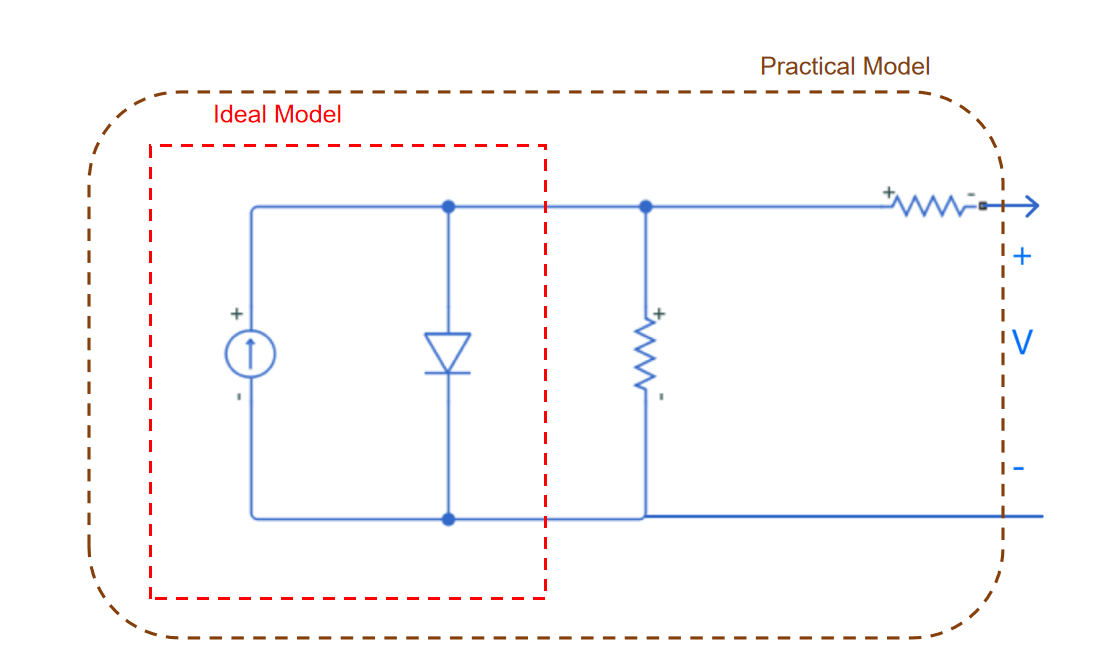
\includegraphics[height=3.5cm]{./images/single diode circuit}
	\caption{single diode circuit}
\end{figure}
\subsection{operation principle of a MPPT system}
Solar power-voltage characteristics' curve is presented in Fig. 1.
\begin{figure}[h]
	\centering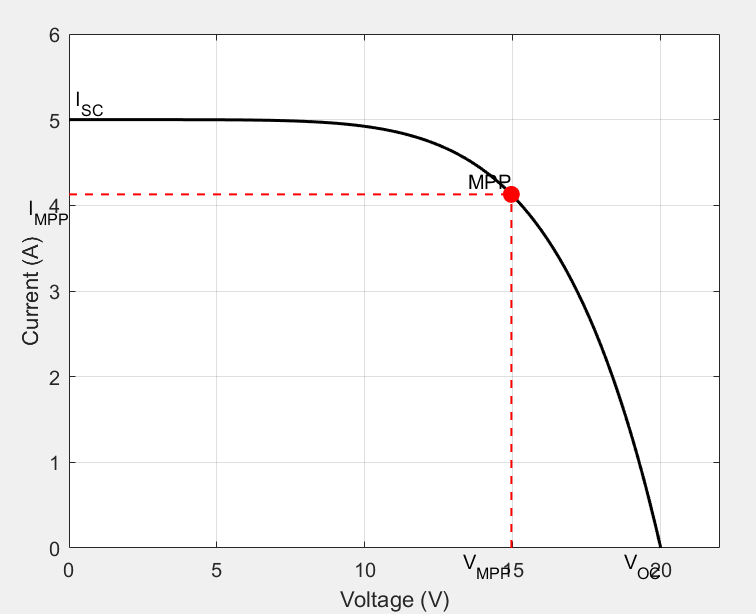
\includegraphics[height=4cm]{./images/current-voltage}
	\caption{current-voltage}
\end{figure}
The MPP is created near the top of the P-V curve, or the famous knee point of the P-V curve, where the generated PV power is maximized. As the MPP depends on solar radiation (S) and temperature (T), and these environmental conditions vary randomly, the MPP position is continuously changed. In order to ensure the operation point is always on the maximum power point, or near it, specific circuits, called MPP trackers, are employed. The DC-DC also applies the controller signal and brings the output to the desired level. Thus, by measuring different parameters (voltage, current or temperature), the maximum power point tracking algorithms calculate the optimal duty cycle (D) and deliver it to the converter to increase the power. Figure 2.3 shows the overview of PV system.
As it is known, the MPP system must operate continuously in real time because the parameters to which the system depends (temperature and radiation) change throughout the day. Changes in the amount of radiations and temperature during the day are  perfectly normal or there may be partial shading. As a result, duty cycle needs to be updated accurately and rapidly (as appropriate).

\begin{figure}[h]
	\centering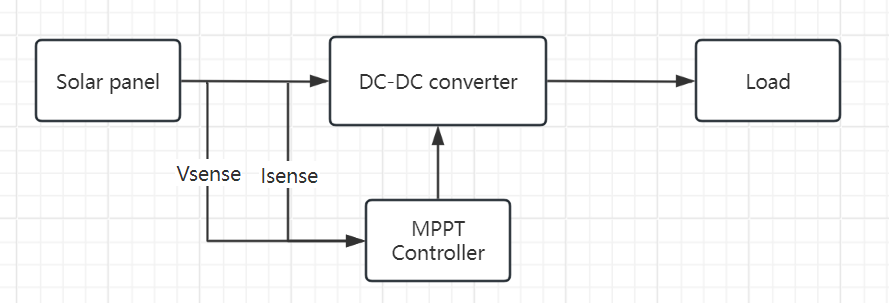
\includegraphics[height=3cm]{./images/Implementation of MPPT system}
	\caption{Implementation of MPPT system}
\end{figure}


\section{Materials}



Important: do not provide results in this section.


	\chapter{Implementation}


Important: do not provide results in this section.

\section{Hardware implementation}

\subsection{DC-DC converter}
The presence of a DC-DC converter leads in control and adjustment of the unregulated DC voltage of output voltage to optimal voltage. The advantages of presence of a DC-DC converter include increase or decrease the dc voltage and adjusting the output voltage according to load changes. These benefits are possible with change of the duty cycle (D). Depending on their output voltage value, different DC-DC converter configurations exist in literature boost, buck, buck-boost, flyback, forward, half and full bridge and etc.


\section{Software implementation}

[TEXT]

	\chapter{Evaluation and validation}

Important: do not introduce new designs, materials or implementation methods in this section.

\begin{table}[h]\centering
    \caption{An example table}
	\begin{tabular}{|l|c|c|}
		\hline
		Day & Min Temp ($^{\circ}$C) & Max Temp ($^{\circ}$C) \\ \hline
		Monday & 11 & 22 \\ \hline
		Tuesday & 9 & 19 \\ \hline
		Wednesday & 10 & 21 \\
		\hline
	\end{tabular}
	\label{tab:exampleTable}
\end{table}
	\chapter{Discussion}

Critical reflection is important in this chapter.

	\chapter{Conclusion}

[TEXT]

	%%% Bibliography: references. included from bibliography.bib
	%%% Only referenced items are displayed in the final document
	%\nocite{*}			% if you also want to display the unreferenced items in your bibliografy uncomment this
	\bibliographystyle{apalike}
	\bibliography{bibliography}

	%%% appendices
    \appendix
    \appendixpage
	% when you are using the twocolumn layout for your thesis appendixes may/can be in a 'singlecolumnsection'
\begin{singlecolumnsection}
\chapter{Some extra info}

Delete the appendix if not needed.

\end{singlecolumnsection}

	%%% Apendix from other pdf
%	\chapter{Poster}
%	\includepdf{poster.pdf}

	\backcover
\end{document}
